\anonsection{Цель лабораторной работы}
Лабораторная работа №4 выполняется на основе лабораторной работы №3.
Ее цель – знакомство с возможностями программы Microsoft Project по контролю за ходом реализации проекта.

Команда разработчиков из 16 человек занимается созданием карты города на основе собственного модуля отображения. 
Проект должен быть завершен в течение 6 месяцев. Бюджет проекта: 50 000 рублей

\anonsection{Индивидуальное задание}
Для выполнения лабораторной работы учитывались следующие параметры:
\begin{enumerate}
	\item Дата отчета: 25.04.2023.
	\item Задача <<Разработка 2D графических интерфейсов>> началась на 7 дней позже.
	\item Задача <<Разработка 3D графических интерфейсов>> закончилась на 7 дней позже.
	\item Задача <<Создание заставки>> выполнена на 90\%.
	\item С 1 апреля на неделю ведущего программиста отправили на курсы повышения квалификации, после чего его ЗП увеличилась на 5\%.
	\item Аренда сервера подорожала на 10\%, начиная с 10.04.2023.
	\item Начали проводиться презентации вместо совещаний раз в две недели (1 час), для которых нужны 4 листа А4 общей стоимостью в 50 рублей, в которых принимают участие только те сотрудники, у которых есть задачи на текущей неделе.
\end{enumerate}

\newpage
\anonsection{Выполнение задания}
Для того, чтобы добавить дату отчёта проекта, нужно выбрать дату в меню \textit{Проект} -> \textit{Задать дату отчёта}

На рисунке 1 представлено добавление даты отчёта:
\FloatBarrier
\begin{figure}[h]	
	\begin{center}
		
\includegraphics[height=5cm]{inc/point.png}
	\end{center}
	\captionsetup{justification=centering}
	\caption{Добавление даты отчёта}
\end{figure}
\FloatBarrier 

Чтобы изменить сроки выполнение заданий, требуется выбрать нужные параметры в меню \textit{Задача} -> \textit{Изменить выполнение}.

Результат изменений для задачи 28 представлен на рисунке 2:
\FloatBarrier
\begin{figure}[h]	
	\begin{center}
		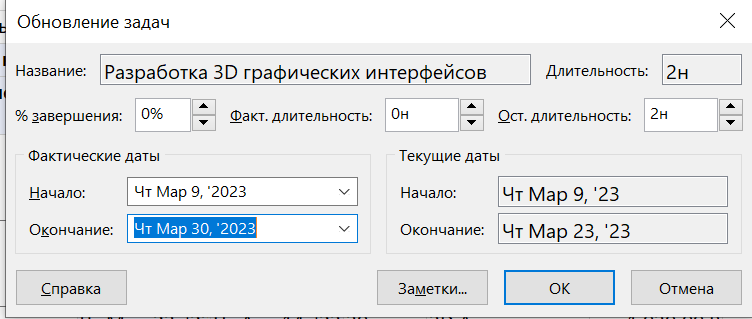
\includegraphics[width=\linewidth]{inc/update2.png}
	\end{center}
	\captionsetup{justification=centering}
	\caption{Изменение сроков выполнения задачи}
\end{figure}
\FloatBarrier 

\newpage
Результат изменений для задачи 29 представлен на рисунке 3:
\FloatBarrier
\begin{figure}[h]	
	\begin{center}
		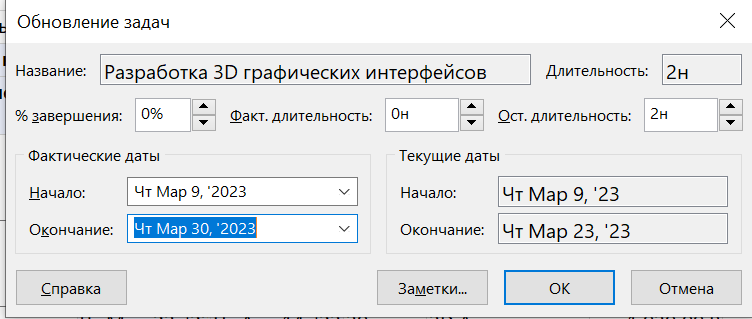
\includegraphics[width=\linewidth]{inc/update2.png}
	\end{center}
	\captionsetup{justification=centering}
	\caption{Изменение сроков выполнения задачи}
\end{figure}
\FloatBarrier 

Результат изменений для задачи 31 представлен на рисунке 4:
\FloatBarrier
\begin{figure}[h]	
	\begin{center}
		
\includegraphics[width=\linewidth]{inc/update3.png}
	\end{center}
	\captionsetup{justification=centering}
	\caption{Изменение процента выполнения задачи}
\end{figure}
\FloatBarrier 

\newpage
Для моделирования ситуации, что ведущий программист ушёл на курсы повышения квалификации, следует изменить доступность ресурса. 
В то время, когда он на курсах, его доступность равна 0\%. 
Изменить это можно на вкладках ресурса.
Результат представлен на рисунке 5:
\FloatBarrier
\begin{figure}[h]	
	\begin{center}
		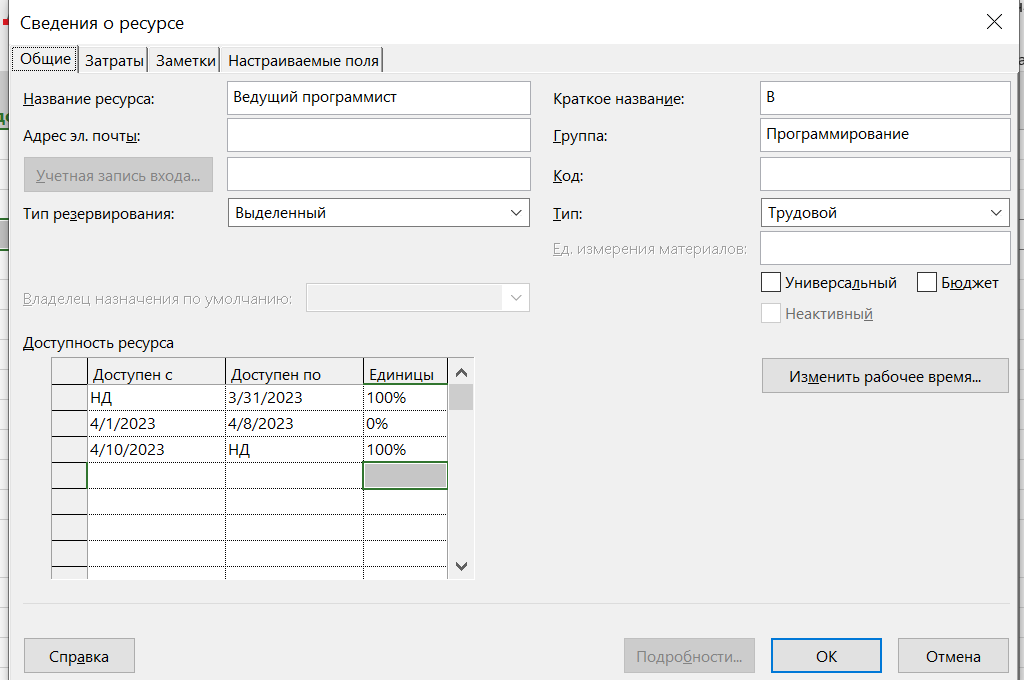
\includegraphics[width=\linewidth]{inc/resurs1.png}
	\end{center}
	\captionsetup{justification=centering}
	\caption{Изменение доступности ведущего программиста}
\end{figure}
\FloatBarrier 

Также его ЗП увеличилась на 5\% по окончанию курса.
В пункте затраты можно указать, с какого момента ЗП будет изменена.
Для того, чтобы смоделировать увеличение, достаточно прописать +5\%, и итоговую сумму MS Project рассчитает автоматически.

\newpage
Результат изменения зарплаты ведущего программиста представлен на рисунке 6:
\FloatBarrier
\begin{figure}[h]	
	\begin{center}
		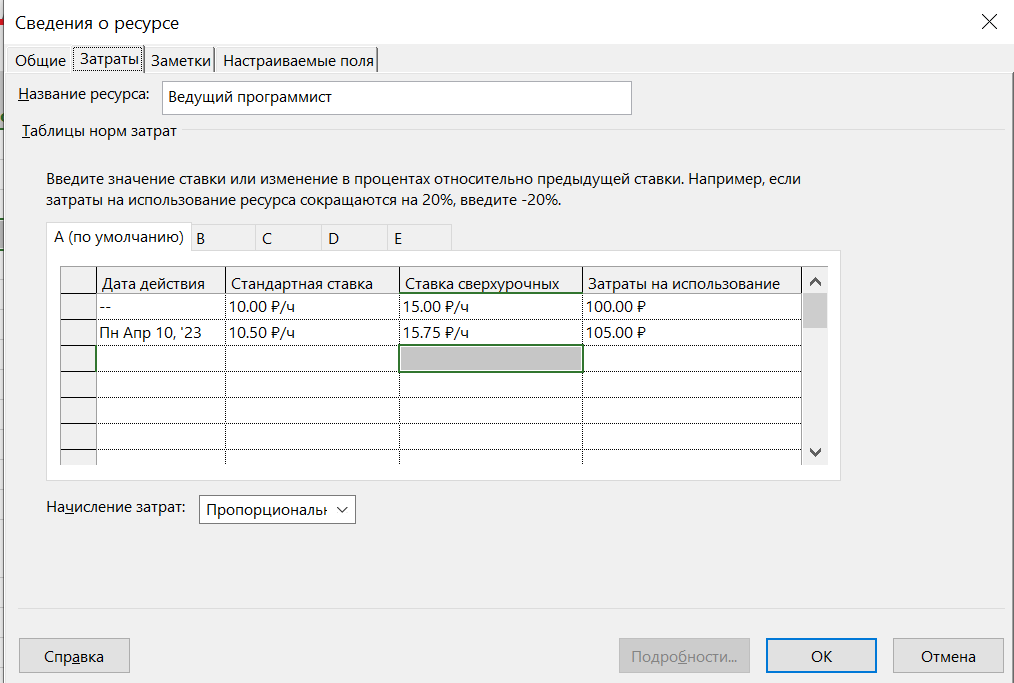
\includegraphics[height=8cm]{inc/resurs2.png}
	\end{center}
	\captionsetup{justification=centering}
	\caption{Изменение зарплаты ведущего программиста}
\end{figure}
\FloatBarrier 

Аналогичные действия были произведены и для сервера. 
Результат представлен на рисунке 7:
\FloatBarrier
\begin{figure}[h]	
	\begin{center}
		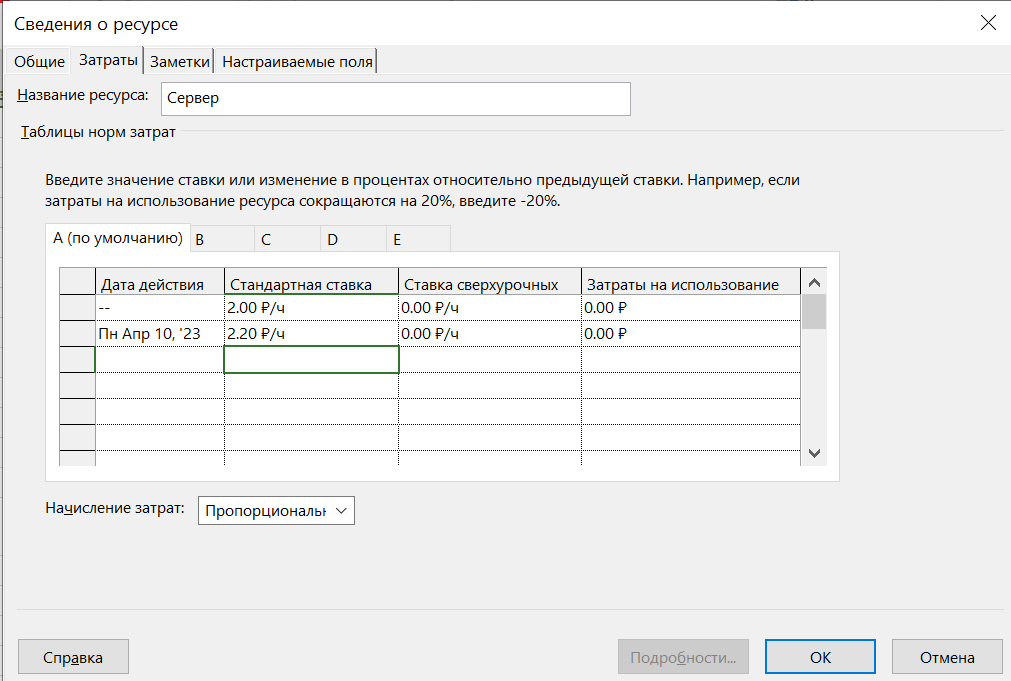
\includegraphics[height=7cm]{inc/server.png}
	\end{center}
	\captionsetup{justification=centering}
	\caption{Изменение трат на сервер}
\end{figure}
\FloatBarrier 
\newpage

Также по заданию требуется добавить новое событие -- презентации, которые с начала апреля заменят обычные совещания и будут проводиться раз в две недели.
Их создание ничем не отличается от создания совещаний.
Также на совещания были назначены ресурсы, в соответствии с тем, кто присутствует на совещании.

Итоговый результат контроля за выполнением представлен на рисунке 8:
\FloatBarrier
\begin{figure}[h]	
	\begin{center}
		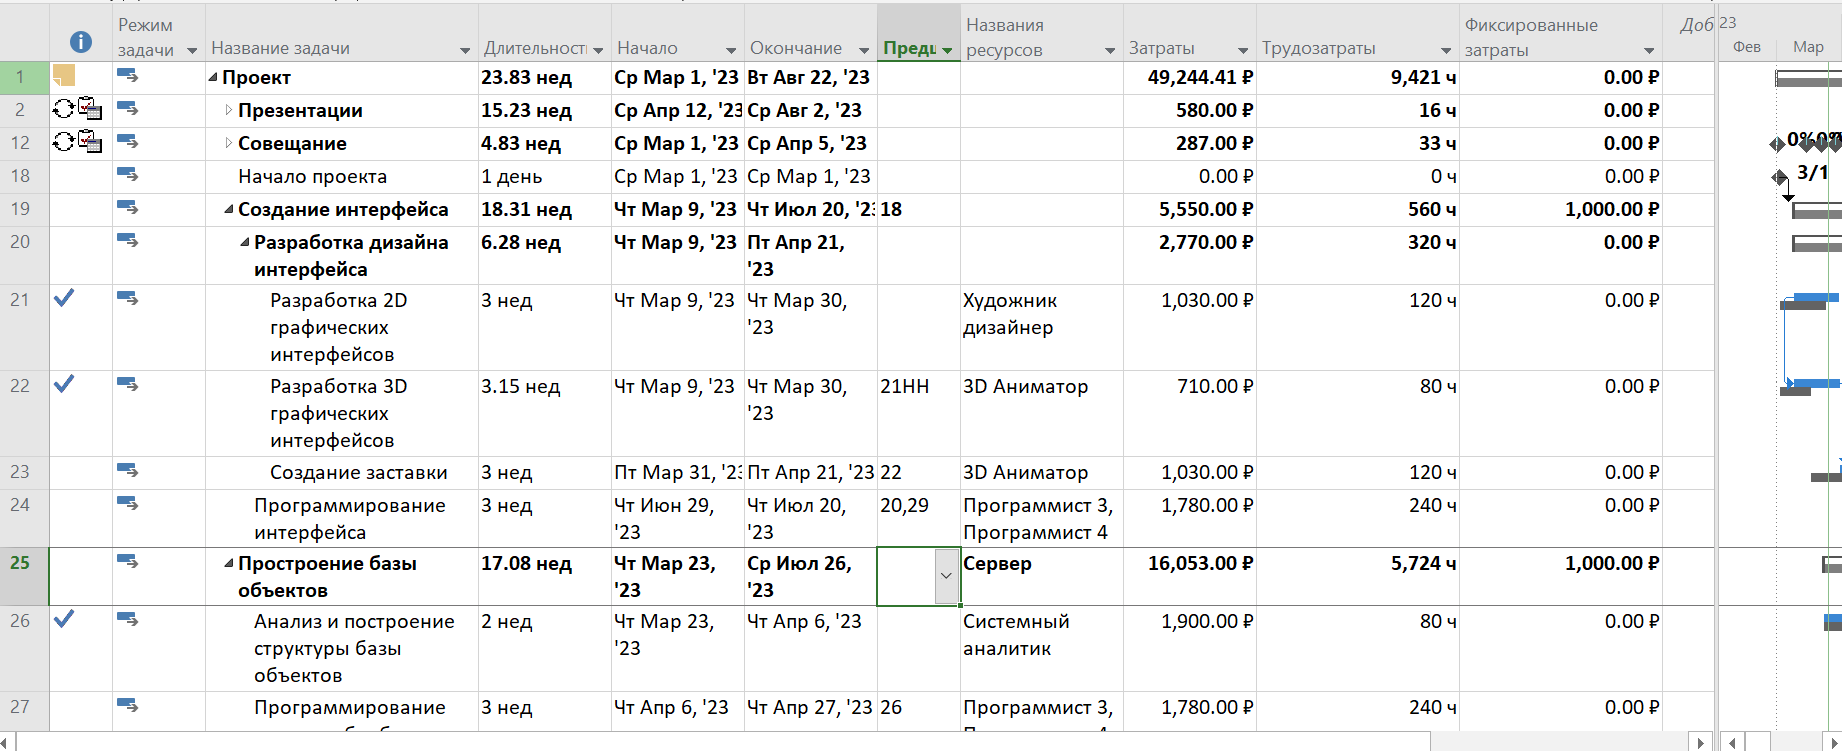
\includegraphics[width=\linewidth]{inc/profit.png}
	\end{center}
	\captionsetup{justification=centering}
	\caption{Результат контроля за выполнением проекта}
\end{figure}
\FloatBarrier 

Можно сделать следующие выводы:
\begin{itemize}
	\item Предполагаемые сроки реализации проекта сдвинулись на одну неделю. Это связано с тем, что ведущий программист одну неделю занимался на курсах повышения квалификации, его задача лежит на критическом пути.
	\item Несмотря на то, что выполнение сроков заданий, связанным с дизайном, оказалось затянутым, это не повлияло на сроки реализации проекта, так как эти задачи не лежат на критическом пути.
	\item Сумма проекта увеличилась с 49004 рублей до 49244 рублей. Этому есть несколько причин: увеличение платы за сервер, повышение зарплаты ведущему программисту. Но презентации проводятся раз в две недели, и чаще всего на нём присутствует только 1-2 человека, соответственно, здесь удалось сэкономить, даже несмотря на 50 рублей расходов на бумагу.
\end{itemize}

\newpage
Диаграмма Ганта представлена на рисунке 9. Здесь также выведены линии реализации проекта.
\FloatBarrier
\begin{figure}[h]	
	\begin{center}
		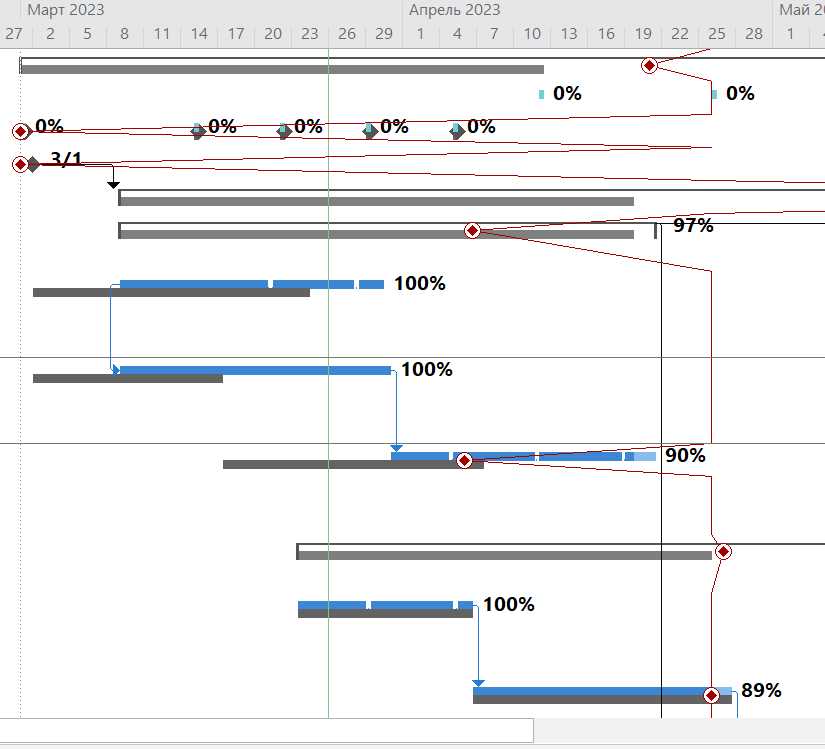
\includegraphics[width=\linewidth]{inc/gant.png}
	\end{center}
	\captionsetup{justification=centering}
	\caption{Диаграмма Ганта}
\end{figure}
\FloatBarrier

\newpage
Так как сроки затянулись на одну неделю, требуется оптимизировать критический путь.
Для этого можно на задачу <<Программирование интерфейсов>> назначить и ведущего программиста.
В этом случае эта задача будет решена по плану на неделю раньше, соответственно, сроки снова сдвинутся до 15 августа.

Итоговый результат после оптимизации представлен на рисунке 10:
\FloatBarrier
\begin{figure}[h]	
	\begin{center}
		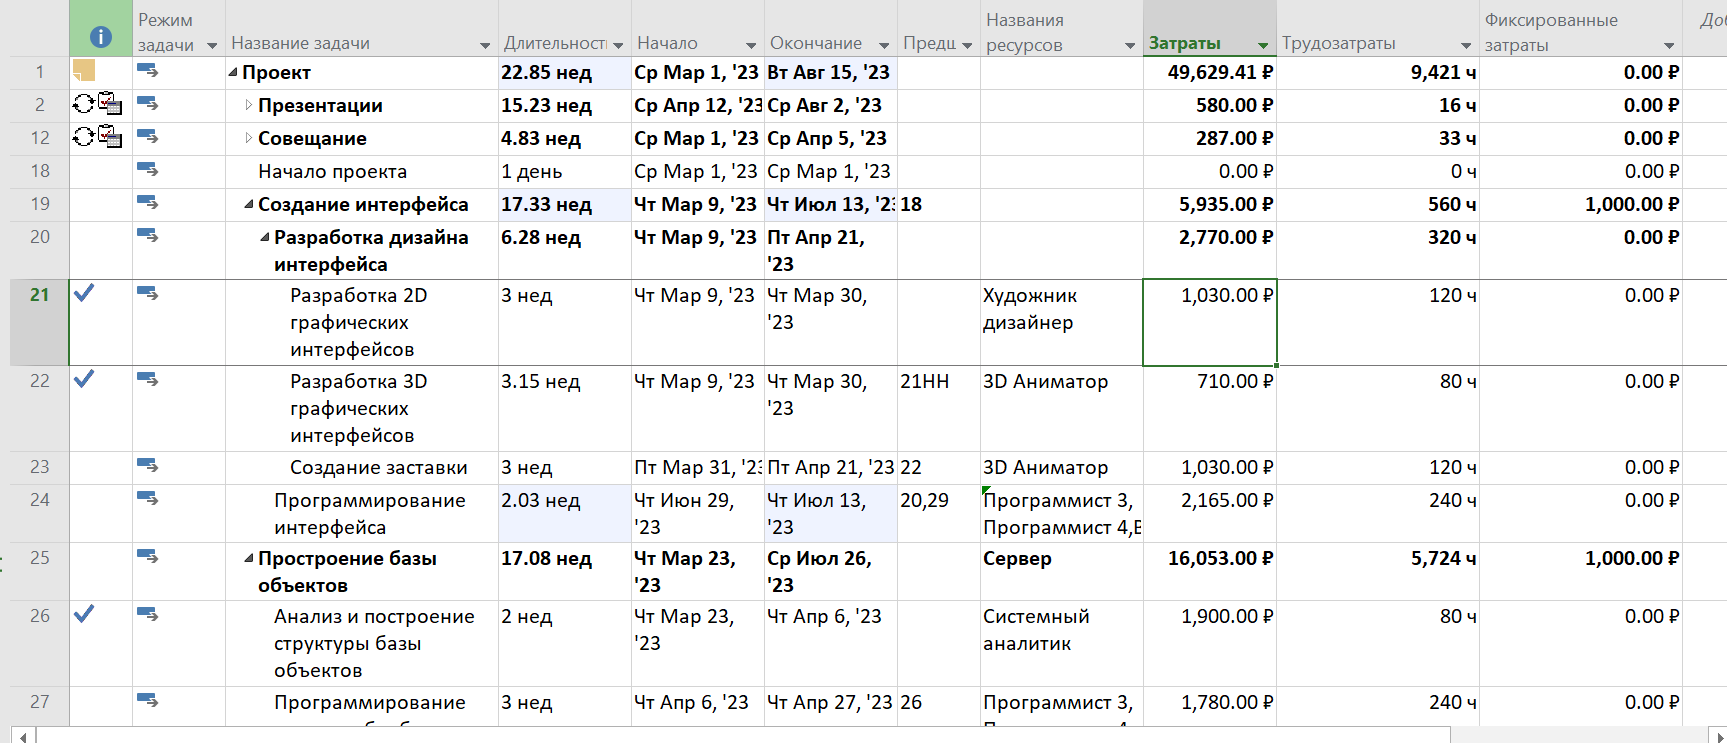
\includegraphics[width=\linewidth]{inc/total.png}
	\end{center}
	\captionsetup{justification=centering}
	\caption{Результат}
\end{figure}
\FloatBarrier

\anonsection{Выводы}
В ходе лабораторной работы удалось провести контроль за выполнением проекта.
Для нескольких задач были добавлены актуальные сроки реализации. 
Выяснилось, что затронутые задачи не лежат на критическом пути, но при этом из-за ведущего программиста выросли затраты, а сроки сдвинулись на одну неделю.

Была добавлена новая повторяющаяся задача -- презентации.
По итогам контроля была построена диаграмма Ганта.

Для того, чтобы ускорить разработку проекта, ведущий программист был привлечен к другой задаче -- <<Программирование интерфейсов>>.

Итоговый результат по проекту: предполагаемый срок сдачи -- 15 августа, расход -- 49629 рублей.
Это соответствует бюджету проекта.